%%%%%%%%%%%%%%%%%%%%%%%%%%%%%%%%%%%%%%%%%
% Beamer Presentation
% LaTeX Template
% Version 1.0 (10/11/12)
%
% This template has been downloaded from:
% http://www.LaTeXTemplates.com
%
% License:
% CC BY-NC-SA 3.0 (http://creativecommons.org/licenses/by-nc-sa/3.0/)
%
%%%%%%%%%%%%%%%%%%%%%%%%%%%%%%%%%%%%%%%%%

%----------------------------------------------------------------------------------------
%	PACKAGES AND THEMES
%----------------------------------------------------------------------------------------

\documentclass[aspectratio=169]{beamer}

\mode<presentation> {

\usetheme{CambridgeUS}

}

\usepackage{color}
\usepackage{graphicx} % Allows including images
\usepackage{url}
\usepackage{hyperref}
\usepackage{algorithm2e}
\usepackage{tikz}

\usetikzlibrary{automata,positioning,arrows,chains,fit,shapes}

\DontPrintSemicolon

\DeclareGraphicsExtensions{.png}

\setlength{\parskip}{1em}

\mathchardef\mhyphen="2D

%----------------------------------------------------------------------------------------
%	TITLE PAGE
%----------------------------------------------------------------------------------------

\title[Complexity theory]{QECDT Topics Presentation: Complexity theory} % The short title appears at the bottom of every slide, the full title is only on the title page

\author{Dominic Moylett} % Your name
\institute[University of Bristol] % Your institution as it will appear on the bottom of every slide, may be shorthand to save space
{
University of Bristol \\ % Your institution for the title page
\medskip
\textit{dominic.moylett@bristol.ac.uk} % Your email address
}
\date{\today} % Date, can be changed to a custom date

\begin{document}

\begin{frame}
\titlepage % Print the title page as the first slide
\end{frame}

%----------------------------------------------------------------------------------------
%	PRESENTATION SLIDES
%----------------------------------------------------------------------------------------

%------------------------------------------------
\section{Introduction: What is complexity theory?}
%------------------------------------------------

\begin{frame}
\frametitle{Complexity theory in a nutshell}
\centerline{``How hard can it be?'', {\em Clarkson}}
\end{frame}

\begin{frame}
\frametitle{What is complexity theory?}
Complexity theory is the study of how difficult it is to solve a problem with a computer.
\end{frame}

\begin{frame}
\frametitle{What is complexity theory?}
Complexity theory is the study of how {\color{red} difficult} it is to solve a problem with a computer.

How do we measure difficulty?
\end{frame}

\begin{frame}
\frametitle{What is complexity theory?}
Complexity theory is the study of how difficult it is to solve a {\color{red} problem} with a computer.

What is a problem?
\end{frame}

\begin{frame}
\frametitle{What is complexity theory?}
Complexity theory is the study of how difficult it is to solve a problem with a {\color{red} computer}.

What is a computer?
\end{frame}

\begin{frame}
\frametitle{Structure of part one}
\begin{itemize}
    \item What is a computer?
    \item What is a problem?
    \item How do we measure difficulty?
\end{itemize}
\end{frame}

%------------------------------------------------
\section{What is a computer?}
%------------------------------------------------

\begin{frame}
\frametitle{Our model of a computer}
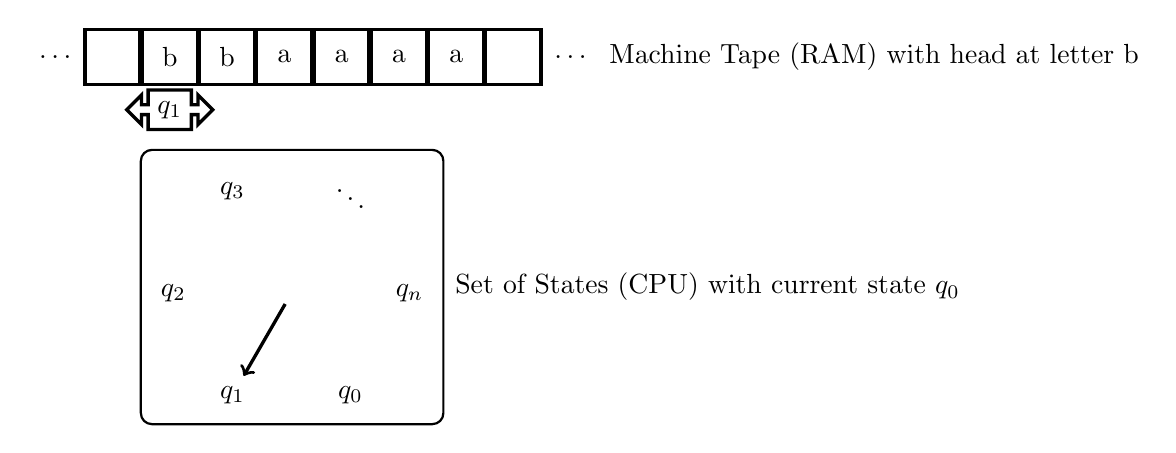
\begin{tikzpicture}
\tikzstyle{every path}=[very thick]

\edef\sizetape{0.7cm}
\tikzstyle{tmtape}=[draw,minimum size=\sizetape]
\tikzstyle{tmhead}=[arrow box,draw,minimum size=.5cm,arrow box
arrows={east:.25cm, west:0.25cm}]

%% Draw TM tape
\begin{scope}[start chain=1 going right,node distance=-0.15mm]
    \node [on chain=1,tmtape,draw=none] {$\ldots$};
    \node [on chain=1,tmtape] {};
    \node [on chain=1,tmtape] (input) {b};
    \node [on chain=1,tmtape] {b};
    \node [on chain=1,tmtape] {a};
    \node [on chain=1,tmtape] {a};
    \node [on chain=1,tmtape] {a};
    \node [on chain=1,tmtape] {a};
    \node [on chain=1,tmtape] {};
    \node [on chain=1,tmtape,draw=none] {$\ldots$};
    \node [on chain=1] {Machine Tape (RAM) with head at letter b};
\end{scope}

%% Draw TM Finite Control
\begin{scope}
[shift={(3cm,-3cm)},start chain=circle placed {at=(-\tikzchaincount*60:1.5)}]
\foreach \i in {q_0,q_1,q_2,q_3,\ddots,q_n}
	\node [on chain] {$\i$};

% Arrow to current state
\node (center) {};
\draw[->] (center) -- (circle-2);

\node[rounded corners,draw=black,thick,fit=(circle-1) (circle-2) (circle-3) 
      (circle-4) (circle-5) (circle-6),
			label=right:Set of States (CPU) with current state $q_0$] (fsbox)
		{};
\end{scope}

%% Draw TM head below (input) tape cell
\node [tmhead,yshift=-.3cm] at (input.south) (head) {$q_1$};

\end{tikzpicture}\footnote{Original version at \url{http://www.texample.net/tikz/examples/turing-machine-2/}}
\end{frame}

\begin{frame}
\frametitle{Formal definition of a computer}
A Turing Machine $(TM)$ is specified as a tuple of seven components $\langle Q, \Gamma, b, \Sigma, q_0, F, \delta \rangle$:

\begin{itemize}
	\item $Q$ is the set of all possible states
	\item $\Gamma$ is tape alphabet
	\item $b \in \Gamma$ is the blank symbol for the tape
	\item $\Sigma = \Gamma/b$ is the input alphabet for the tape
	\item $q_0 \in Q$ is the start state
	\item $F \subseteq Q$ is the set of accepting states
	\item $\delta: Q \times \Gamma \to Q \times \Sigma \times \{L, R\}$ is the transition function
\end{itemize}
\end{frame}

\begin{frame}
\frametitle{But how do we run it?}
The majority of computation time is spent repeating the following loop. Note that $T_h$ is the $h$-th cell of the tape.
\begin{algorithm}[H]
$q = q_0$\\
$h = 0$\\
$T = w$ \tcp*{Tape starts as just input, followed by blank cells}
\While{$\delta(q, T_h)$ is not undefined}{
	$(q, h, i) = \delta(q, T_h)$\\
	\eIf{$i = L$}{$h = h - 1$ \tcp*{Move tape head to the left}}
	{$h = h + 1$ \tcp*{Move tape head to the right}}
}
\end{algorithm}
\end{frame}

\begin{frame}
\frametitle{What happens when it stops?}
When we reach a point that $\delta(q, T_h)$ undefined, the machine has {\em halted}. What happens next depends on the state the machine stopped in.
\begin{algorithm}[H]
\eIf{$q \in F$}{\bf{accept}\\\bf{return} $T$ \tcp*{This is thought of as the output of $M(w)$}}
{\bf{reject}}
\end{algorithm}
\end{frame}

\begin{frame}
\frametitle{What can we store in a machine's memory?}
\begin{itemize}
	\item<1-> Integers
	\item<2-> Rational numbers
	\item<3-> Floating point numbers
	\item<4-> Boolean (True/False) statements
	\item<5-> Text
	\item<6-> Other machines
\end{itemize}
\end{frame}

\begin{frame}
\frametitle{Universal Turing Machines}
Turing showed in his PhD thesis that we could represent the current state of any $TM$ -- including current state, tape and position of tape head -- as an integer.

Not only that, but we could manipulate this integer such that it matched performing the next step of the computation.

This gave way to Universal Turing Machines; machines capable of running any $TM$ given to them.
\end{frame}

\begin{frame}
\frametitle{The Church-Turing Thesis}
\centerline{``[A]ll effectively calculable sequences are computable'', {\em Turing}}
\end{frame}

\begin{frame}
\frametitle{Quiz Time!}

\begin{center}
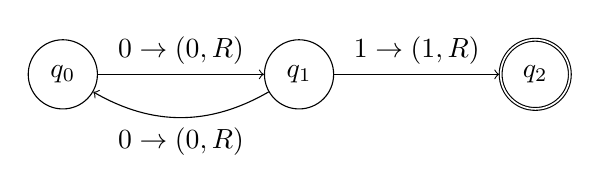
\begin{tikzpicture}[node distance=3cm,on grid,auto]
    \node[state] (q0) at (0,0) {$q_0$};
    \node[state] (q1) [right of=q0] {$q_1$};
    \node[accepting,state] (q2) [right of=q1] {$q_2$};
    \path[->]
        (q0) edge node {$0 \to (0, R)$} (q1)
        (q1) edge node {$1 \to (1, R)$} (q2)
        (q1) edge [bend left] node {$0 \to (0, R)$} (q0);
\end{tikzpicture}
\end{center}

$q_0$ is the start state, and $q_2$ is the accept state.

Question: Does $M(01)$ {\bf accept} or {\bf reject}?
\end{frame}

\begin{frame}
\frametitle{Quiz Time!}

\begin{center}
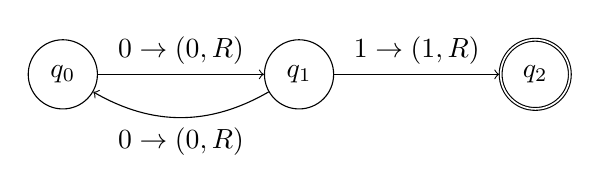
\begin{tikzpicture}[node distance=3cm,on grid,auto]
    \node[state] (q0) at (0,0) {$q_0$};
    \node[state] (q1) [right of=q0] {$q_1$};
    \node[accepting,state] (q2) [right of=q1] {$q_2$};
    \path[->]
        (q0) edge node {$0 \to (0, R)$} (q1)
        (q1) edge node {$1 \to (1, R)$} (q2)
        (q1) edge [bend left] node {$0 \to (0, R)$} (q0);
\end{tikzpicture}
\end{center}

$q_0$ is the start state, and $q_2$ is the accept state.

Answer: $M(01)$ {\bf accept}s!
\end{frame}

\begin{frame}
\frametitle{Quiz Time!}

\begin{center}
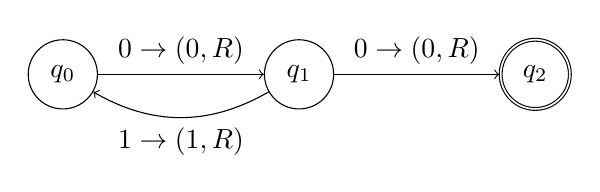
\begin{tikzpicture}[node distance=3cm,on grid,auto]
    \node[state] (q0) at (0,0) {$q_0$};
    \node[state] (q1) [right of=q0] {$q_1$};
    \node[accepting,state] (q2) [right of=q1] {$q_2$};
    \path[->]
        (q0) edge node {$0 \to (0, R)$} (q1)
        (q1) edge node {$0 \to (0, R)$} (q2)
        (q1) edge [bend left] node {$1 \to (1, R)$} (q0);
\end{tikzpicture}
\end{center}

$q_0$ is the start state, and $q_2$ is the accept state.

Question: Does $M(01)$ {\bf accept} or {\bf reject}?
\end{frame}

\begin{frame}
\frametitle{Quiz Time!}

\begin{center}
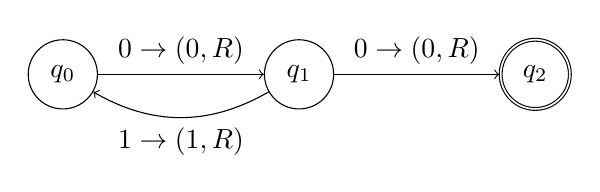
\begin{tikzpicture}[node distance=3cm,on grid,auto]
    \node[state] (q0) at (0,0) {$q_0$};
    \node[state] (q1) [right of=q0] {$q_1$};
    \node[accepting,state] (q2) [right of=q1] {$q_2$};
    \path[->]
        (q0) edge node {$0 \to (0, R)$} (q1)
        (q1) edge node {$0 \to (0, R)$} (q2)
        (q1) edge [bend left] node {$1 \to (1, R)$} (q0);
\end{tikzpicture}
\end{center}

$q_0$ is the start state, and $q_2$ is the accept state.

Answer: $M(01)$ {\bf reject}s!
\end{frame}

\begin{frame}
\frametitle{Quiz Time!}

\begin{center}
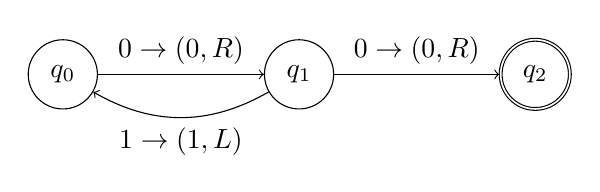
\begin{tikzpicture}[node distance=3cm,on grid,auto]
    \node[state] (q0) at (0,0) {$q_0$};
    \node[state] (q1) [right of=q0] {$q_1$};
    \node[accepting,state] (q2) [right of=q1] {$q_2$};
    \path[->]
        (q0) edge node {$0 \to (0, R)$} (q1)
        (q1) edge node {$0 \to (0, R)$} (q2)
        (q1) edge [bend left] node {$1 \to (1, L)$} (q0);
\end{tikzpicture}
\end{center}

$q_0$ is the start state, and $q_2$ is the accept state.

Question: Does $M(01)$ {\bf accept} or {\bf reject}?
\end{frame}

\begin{frame}
\frametitle{Quiz Time!}

\begin{center}
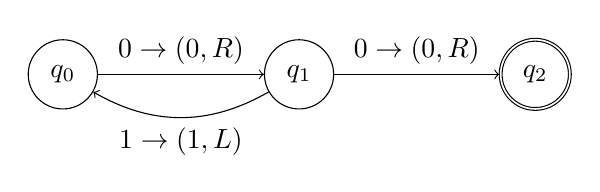
\begin{tikzpicture}[node distance=3cm,on grid,auto]
    \node[state] (q0) at (0,0) {$q_0$};
    \node[state] (q1) [right of=q0] {$q_1$};
    \node[accepting,state] (q2) [right of=q1] {$q_2$};
    \path[->]
        (q0) edge node {$0 \to (0, R)$} (q1)
        (q1) edge node {$0 \to (0, R)$} (q2)
        (q1) edge [bend left] node {$1 \to (1, L)$} (q0);
\end{tikzpicture}
\end{center}

$q_0$ is the start state, and $q_2$ is the accept state.

Answer: $M(w)$ doesn't halt. This can be interpreted as rejection, depending on how the problem is phrased.
\end{frame}

\begin{frame}
\frametitle{The halting problem}
You might think it would be useful if we could tell when a machine was going to halt.

Formally, we would want a $TM\, H$, such that given $M \in TM \text{ and } w \in \Sigma_M^*$:

\begin{itemize}
	\item $H(M, w)$ halts in the {\bf accept} state if $M(w)$ halts and
	\item $H(M, w)$ halts in the {\bf reject} state if $M(w)$ does not halt.
\end{itemize}

Sadly, Turing proved that such a machine is impossible.

There are many other unsolvable problems as well, within the area of {\bf computability theory}. We will not cover this area, but some reading on the subject is suggested at the end.
\end{frame}

\begin{frame}
\frametitle{Nondeterminism: Spot the difference!}
A Nondeterministic Turing Machine $(NTM)$ is specified as a tuple of seven components $\langle Q, \Gamma, b, \Sigma, q_0, F, \delta \rangle$:

\begin{itemize}
	\item $Q$ is the set of all possible states
	\item $\Gamma$ is tape alphabet
	\item $b \in \Gamma$ is the blank symbol for the tape
	\item $\Sigma = \Gamma/b$ is the input alphabet for the tape
	\item $q_0 \in Q$ is the start state
	\item $F \subseteq Q$ is the set of accepting states
	\item $\delta: Q \times \Gamma \to (Q \times \Sigma \times \{L, R\})^*$ is the transition function
\end{itemize}
\end{frame}

\begin{frame}
\frametitle{What, what's the difference?}
$NTM$s are different because of the transition function.

In deterministic $TMs$, the transition goes from one machine setup to another.

In $NTM$s, the transition function goes from one to many setups.

These setups are run simultaneously, and the machine accepts if one setup halts in an accepting state, or rejects if all setups halt in the rejecting state.
\end{frame}

\begin{frame}
\frametitle{Computation Tree}

\end{frame}

\begin{frame}
\frametitle{Power of Nondeterminism}
Note that a $TM$s only transition from one machine setup to another, while $NTM$s transition from one to many.

From this, we can conclude that any $TM$ is by definition also an $NTM$.

Question: Do $NTM$s violate the Church-Turing Thesis? Or put another way, is there any problem that can be solved by an $NTM$ that cannot be solved by a $TM$?
\end{frame}

\begin{frame}
\frametitle{Using $TM$s to simulate $NTM$s}
Recall the computation tree:

We can use a technique called Breadth-First Search to search every branch until we find one that halts in an {\bf accept} state.

Note that this does not mean we can simulate NTMs easily...
\end{frame}

%------------------------------------------------
\section{Summary of part one}
%------------------------------------------------

\begin{frame}
\frametitle{Summary of part one}
\begin{itemize}
    \item What is a computer? {\em Deterministic Turing Machine, Non-Deterministic Turing Machine}
    \item What is a problem? {\em Deciding if a word is in a language, verifying that a word is in a language}
    \item How do we measure difficulty? {\em Upper bound of time for an input of length $n$}
\end{itemize}
\end{frame}

%------------------------------------------------
\section{End of part one}
%------------------------------------------------

\begin{frame}
\frametitle{End of part one}
\begin{center}
\includegraphics{turing_comic}\footnote{\url{http://www.cs.utah.edu/~draperg/cartoons/2005/turing.html}}
\end{center}
\end{frame}

%------------------------------------------------
\section{Structure of part two}
%------------------------------------------------

\begin{frame}
\frametitle{Structure of part two}
\begin{itemize}
    \item Putting it all together!
    \item ...only to get another (very difficult) problem.
    \item How might we try to solve this new problem?
\end{itemize}
\end{frame}

%------------------------------------------------
\section{The $P$ versus $NP$ problem}
%------------------------------------------------

\begin{frame}
\frametitle{Pop quiz!}
\centerline{Does $P=NP$?}
\end{frame}

\begin{frame}
\frametitle{The $P$ versus $NP$ problem}
Arguably first proposed by G\"{o}del in a letter to von Neumann in 1956.\footnote{\url{https://ecommons.cornell.edu/bitstream/handle/1813/6910/89-994.pdf}}

First stated formally by Cook in 1971.\footnote{\url{http://dl.acm.org/citation.cfm?coll=GUIDE&dl=GUIDE&id=805047}}

Solving the problem will earn you a million dollars, courtesy of the Clay Mathematics Institute.\footnote{\url{http://www.claymath.org/millennium-problems/p-vs-np-problem}}
\end{frame}

\begin{frame}
\frametitle{The easy side: $P \subseteq NP$}

Recall that any $TM$ is by definition non-deterministic.

Likewise, any polynomial-time $TM$ is also non-deterministic.

Hence $P \subseteq NP$.
\end{frame}

\begin{frame}
\frametitle{The easy side: $P \subseteq NP$}

Alternative proof (using verification):

Let $TM\, M$ decide $L$ in polynomial time. Define $V$ as follows:

\begin{algorithm}[H]
$V(w, c):$\\
\If{$M(w)$ accepts}{
    {\bf accept}
}
\Else{
    {\bf reject}
}
\end{algorithm}

$V$ verifies $L$ in polynomial time. Hence $P \subseteq NP$.
\end{frame}

\begin{frame}
\frametitle{The harder side: Is $NP \subseteq P$}

Another way to think of this problem: {\em If a problem can be easily verified, can it be easily solved?}
\end{frame}

\begin{frame}
\frametitle{How might we answer this question?}

Why not look at the hardest problems in $NP$?

If $P = NP$, then even the hardest problems in $NP$ will be solvable in polynomial time.

And if $P \subset NP$, then these are the problems that won't have a polynomial time solution, as could be checked by lower-bound analysis.

But how can we determine the hardest problems in $NP$?
\end{frame}

%------------------------------------------------
\section{Summary of part two}
%------------------------------------------------

\begin{frame}
\frametitle{Summary of part two}
\begin{itemize}
    \item Putting it all together! {\em $P, NP$}
    \item ...only to get another (very difficult) problem. {\em Are easy to verify problems easy to solve?}
    \item How might we try to solve this new problem? {\em $NP\mhyphen Complete$ problems}
\end{itemize}
\end{frame}

%------------------------------------------------
\section{Beyond $P$ and $NP$}
%------------------------------------------------

\begin{frame}
\frametitle{What else is there?}
Recall our three questions from part one:
\begin{itemize}
    \item What is a computer?
    \item What is a problem?
    \item How do we measure difficulty?
\end{itemize}
What if we answered these differently?
\end{frame}

\begin{frame}
\frametitle{What is a computer?}
Probabilistic Turing Machines: $BPP, RP$

Parallel Computing: $NC$

Talking to another, more powerful computer: $MA, IP$

Quantum computers:  $EQP, BQP$

Time travel: $P_{CTC}$
\end{frame}

\begin{frame}
\frametitle{What is a problem?}
Computational problems: $NP\mhyphen Hard$

Counting problems: $\#P$

Complementary problems: $co\mhyphen NP$
\end{frame}

\begin{frame}
\frametitle{How do we measure difficulty?}
Exponential time: $EXP$

Linear time: $LIN$

Space complexity: $PSPACE, EXPSPACE$

Sublinear working space: $L$
\end{frame}

\begin{frame}
\frametitle{This is only the beginning}
There are many more complexity classes out there, and very quickly relating them in a simple equation like this:

$$P \subseteq NP$$

Becomes this:

$$L \subseteq NL \subseteq P \subseteq NP \subseteq PSPACE = NPSPACE = IP = P_{CTC} \subseteq EXP \subseteq EXPSPACE$$
\end{frame}

%------------------------------------------------
\section{The end}
%------------------------------------------------

\begin{frame}
\begin{center}
\frametitle{The end}
\includegraphics[scale=0.2]{smbc_comic}\footnote{\url{http://www.smbc-comics.com/?id=3919}}
\end{center}
\end{frame}

\begin{frame}
\begin{center}
\frametitle{The end}
\includegraphics[scale=0.5]{smbc_comic_votey}\footnote{\url{http://www.smbc-comics.com/?id=3919}}
\end{center}
\end{frame}

%----------------------------------------------------------------------------------------

\end{document} 
